El protocolo \gls{NETCONF} es un protocolo de gestión de redes desarrollado y estandarizado por la \gls{IETF}. Fue desarrollado en el grupo de trabajo NETCONF publicado en diciembre de 2006 en el \rfclink{RFC4741} y posteriormente revisado en junio 2011 en el \rfclink{RFC6241}. 

\gls{NETCONF} proporciona los mecanispos para instalar, manipular y borrar la configuración de dispositivos de red. Las operaciones del protocolo \gls{NETCONF} se realizan mediante \glspl{RPC} y usan una codificación \gls{XML} tanto para los datos que constituyen la configuración como para los mensajes del propio protocolo. 

El protocolo se puede dividir conceptualmente en cuatro capas que se pueden ver en la Figura \ref{fig:capas_netconf}:
\begin{itemize}
    \item \textbf{Transporte}: La capa de transporte proporciona un canal de comunicación entre el cliente y el servidor.
    \item \textbf{Mensajes}: La capa de mensajes proporciona una forma simple, para enmarcar y codificar los mensajes del protocolo.
    \item \textbf{Operaciones}: La capa de operaciones define el conjunto de operaciones básicas y sus parámetros.
    \item \textbf{Contenido}: Define la organización y el modelado de los datos de configuración.
\end{itemize}

\begin{figure}
    \centering
    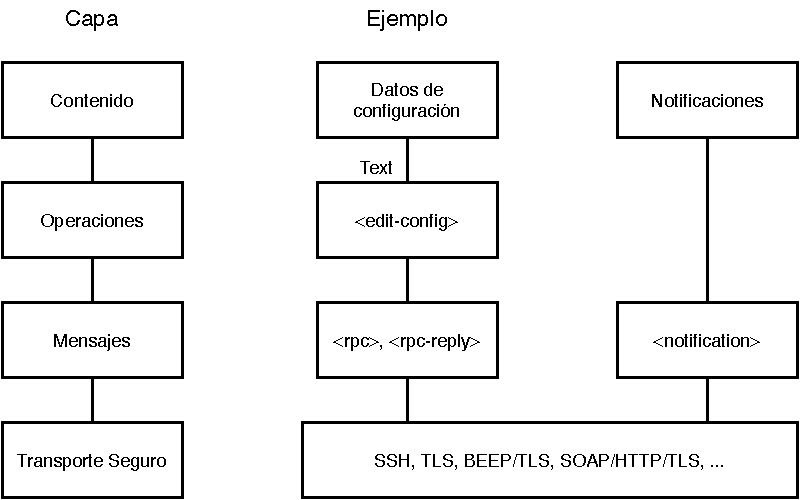
\includegraphics[scale=.75]{graphics/Capas_Netconf.pdf}
    \caption{Capas del protocolo \gls{NETCONF}}
    \label{fig:capas_netconf}
\end{figure}

\subsubsection{Transporte}

\gls{NETCONF} usa mensajes \glspl{RPC} para comunicarse. Un cliente manda una serie de solicitudes \gls{RPC} que provocan el el servidor responda con una serie de respuestas RPC. \gls{NETCONF} puede usar cualquier protocolo de transporte siempre que este proporcione la funcionalidad necesaria:

\begin{itemize}
    \item \textbf{Orientado a conexión}: \gls{NETCONF} requiere una conexión persistente entre pares.
    \item \textbf{Autenticación, Integridad y Confidencialidad}
\end{itemize}

Aunque existe soporte para muchos protocolos de transporte, los más usados son \gls{NETCONF} sobre \gls{SSH} \rfclink{RFC6242}\cite{RFC6242} y \gls{NETCONF} sobre \gls{TLS} con Autenticación mutua usando certificados X.509 \rfclink{RFC7589}\cite{RFC7589}.

\subsubsection{Mensajes}
La base del protocolo \gls{NETCONF} proporciona tres tipos de mensajes:

\begin{itemize}
    \item Solicitudes \gls{RPC} (mensajes <rpc>)
    \item Respuestas \gls{RPC} (mensajes <rpc-reply>)
    \item Notificaciones de eventos (mensajes <notification>)
\end{itemize}

Cada mensaje del protocolo \gls{NETCONF} es un documento \gls{XML} bien formado y codificado usando UTF-8. Las solicitudes y las respuestas se relacionan entre si mediante un atributo \enquote{message-id} de forma que el protocolo \gls{NETCONF} permite el \enquote{pipelining} de mensajes.

\subsubsection{Operaciones}

El protocolo \gls{NETCONF} proporciona un conjunto pequeño de operaciones de bajo nivel para gestionar la configuración de los dispositivos y recuperar información de estado. El protocolo base proporciona operaciones para recuperar, configurar, copiar y borrar elementos de configuración. Otras operaciones se pueden añadir en función de las capacidades anunciadas por el dispositivo. Las operaciones básicas son:

\begin{itemize}
    \item \textbf{get}: Recupera la configuración y la información de estado del dispositivo. A diferencia de \enquote{get-config} también puede recuperar información de estado.
    \item \textbf{get-config}: Recupera todo o parte de un datastore de configuración especifico. 
    \item \textbf{edit-config}: Carga todo o parte de una configuración a un datastore especifico.
    \item \textbf{copy-config}: Crea o reemplaza un datastore completo con los contenidos de otro datastore.
    \item \textbf{delete-config}: Elimina un datastore de configuración. El almacén de datos \enquote{running} no puede ser eliminado.
    \item \textbf{lock}: Permite a un cliente bloquear temporalmente un almacén de datos con el fin de realizar cambios sin interacciones por parte de otros clientes NETCONF.
    \item \textbf{unlock}: Libera el bloqueo iniciado por una operación \enquote{lock} permitiendo de nuevo realizar modificaciones sobre el datastore afectado.
    \item \textbf{close-session}: Solicita la finalización de forma elegante de una sesión de \gls{NETCONF}.
    \item \textbf{kill-session}: Fuerza la finalización de una sesión NETCONF
\end{itemize}

\subsubsection{Contenido}

La última revisión del protocolo NETCONF, el \rfclink{RFC6241}\cite{RFC6241} no proporciona una definición para la capa de Contenido, quedando fuera del alcance de dicho documento. Los datos de configuración se definen mediante el lenguaje de modelado de datos YANG que se explicará en la Sección \ref{sec:yang_data_model}.




